\chapter{Нейросетевые модели управления технологическими процессами}

В данной главе рассматриваются практические примеры применения в задачах АСУТП.

\section{Процесс пастеризации молока}

\subsection{Общие сведения}

К концу XIX века тепловая обработка молока получила столь широкое применение, что стала использоваться для разнообразных целей на большинстве молокозаводов – например, для обработки молока при изготовлении сыра и масла. До внедрения тепловой обработки молоко представляло собой постоянный источник инфекций, так как оно является идеальной средой для развития микроорганизмов. Через молоко зачастую распространялись такие болезни, как туберкулез и брюшной тиф.

Перед тем, как перейти к описанию процесса пастеризации необходимо иметь полное понимание о молоке как об объекте технической обработки. Рассматривая его таким образом можно сказать, что оно должно обладать некоторыми показателями и характеристиками, например, состав молока, степень чистоты, кислотность, наличие токсичных и нейтрализующих веществ. Кроме того, молоко обладает ещё и различными свойствами: органолептическими, физико-механическими и биохимическими. Впрочем, достаточно будет разобрать лишь свойства и характеристики, которые необходимы для понимания процесса пастеризации.

Молоко можно разделить на две составляющих: вода и распределённые в этой воде пищевые вещества. К таким веществам относят жиры, белки, углеводы, ферменты, различные минеральные вещества и газы. Помимо этого, о чём говорилось немного ранее, в молоке могут находится различные микроорганизмы. И как известно, некоторые из этих микроорганизмов, содержащиеся в молоке, являются опасными или вредными, например, бруцеллеза, ящура, возбудитель кишечной палочки и другие. Но как избавиться от вредных и опасных микроорганизмов?  Для этого, как раз-таки, и используется процесс пастеризации - уничтожение различных форм вредных и опасных микроорганизмов в молоке, но при этом с сохранением биологической и питательной ценности, а также и качества молока. Такое определение для пастеризации можно вывести относительно того, что происходит с молоком во время этого процесса, а остальные технические и технологические подробности при этом отсутствуют.

Однако перед тем, как перейти к пастеризации как к техническому процессу, необходимо определить, какое молоко подлежит пастеризации, а также каким требованиям оно должно соответствовать. Для определения подходящего перед пастеризацией молока существует множество различных показателей и требований. Так, например, пригодное для пастеризации молоко должно быть кислотностью не более 22 °T, а бактериальная обсеменённость молока должна быть один миллион клеток на сантиметр кубический. При этом, молоко не должно быть вспененным, поскольку пена нарушает теплообмен в ходе пастеризации. А перед самой пастеризацией, молоко должно быть также предварительно очищено на фильтрах или на сепараторах-молокоочистителях. Что ж, основные требования к пригодному для пастеризации молоку перечислены.

В термине “пастеризация” запечатлено имя Луи Пастера, который в середине XIX века провел фундаментальные исследования воздействия тепла на микроорганизмы, приводящего к их гибели, и возможности применения температурной обработки для консервирования пищевых продуктов. Основные параметры пастеризации есть температура пастеризации, а также время выдержки, то есть время нахождения молока в данном процессе. Относительно данных параметров существует выражение, которое называется критерием Пастера. Этот критерий можно рассчитать по формуле:

\begin{equation}
    P=\frac{t}{p}
\end{equation}

где $t$ - время действия температуры пастеризации, с; $p$ - время бактерицидного действия температуры пастеризации - эффект, в результате которого происходит уничтожение вредных и опасных микроорганизмов, с.

Также известна и ещё одна немаловажная зависимость: продолжительность выдержки зависит от температуры пастеризации. Зависимость показана в формуле:

\begin{equation}
    \ln{t} = 36.84 - 048T
\end{equation}

где $T$ {--} температура пастеризации, $^{\circ}$C.

Завершение процесса пастеризации характеризуется полным уничтожением содержащихся в молоке микроорганизмов. Это можно будет определить благодаря уже известному критерию Пастера, значение которого должно быть не меньше единицы, для того чтобы считать, что процесс пастеризации завершён.

Таким образом, пастеризация молока как технологический процесс – это особый вид тепловой обработки, который можно определить как “любую тепловую обработку молока, обеспечивающую безусловное уничтожение микроорганизмов – возбудителей туберкулеза, не вызывая при этом значительных изменений физических и химических качеств молока” \cite{TetraPak1995}.

Пластинчатая пастеризационно-охладительная установка (ПОУ) предназначена для тепловой обработки и охлаждения молочных продуктов в непрерывном тонкослойном закрытом потоке. Схема типовой пастеризационной установки приведена ниже (рис. \ref{fig:POU_Tetra_Pak}). Нагрев осуществляется за счет подачи пара через управляемый клапан \textbf{VC1}. Диапазон работы управляемых паровых клапанов от $\text{0\%}$ – полностью закрыт, до $\text{100\%}$ – полностью открыт. Температура \textbf{TE1} поддерживаться в пределах $92 \pm 2 \SI{}{\celsius}$.

Современная ПОУ, включающая оборудование для эксплуатации, надзора и управления процессом, собирается из согласованных компонентов, образуя сложный технологический агрегат. Для автоматизации регулирования температурного режима в состав ПОУ входит система управления на базе промышленного контроллера. От применяемых алгоритмов управления напрямую зависит качество получаемой продукции.

\begin{figure}[H]
    \centering
    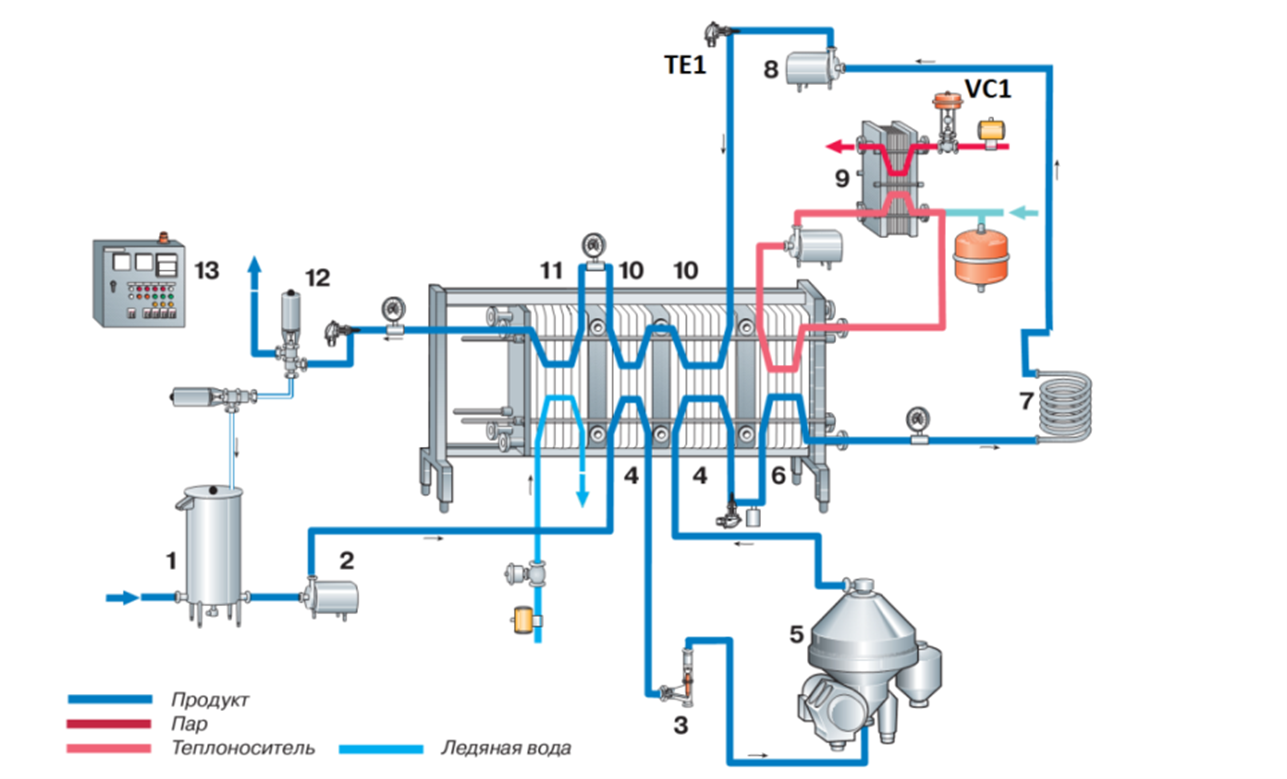
\includegraphics[width=\textwidth]{images/chapter_2/ПОУ Tetra Pak.png}
    \caption{Схема и общий вид пастеризационной установки, где: 1 - балансный танк, 2 - подающий насос, 3 - регулятор потока, 4 - секции регенеративного предварительного подогрева, 5 - центробежный очиститель, 6 - секция нагрева, 7 - труба выдержки, 8 - вспомогательный насос, 9 - система нагрева горячей воды, 10 - секции регенеративного охлаждения, 11 - секции охлаждения, 12 - клапан возвратный, 13 - панель управления}
    \label{fig:POU_Tetra_Pak}
\end{figure}

\subsection{Пастеризационные установки как объект автоматизации}

Коротко разберём каждый элемент ПОУ.

Балансный танк является по сути резервуаром с молоком, оборудованным поплавковым входным клапаном, который регулирует расход молока и поддерживает его постоянный уровень в резервуаре. В балансном танке также имеется электрод минимального уровня. Он срабатывает, в том случае, когда уровень молока достигает минимальной точки, тем самым включая клапан распределения потока. Молоко заменяется водой и пастеризатор отключается.

Подающий насос позволяет обеспечить молоком сам пастеризатор, выкачивая его из балансного танка.

Для обеспечения устойчивого контроля температуры и постоянного времени выдержки пастеризационной установки используется регулятор потока. Он также необходим для поддержки расхода через пастеризатор на должно уровне.

Молоко, попав в секцию подогрева, должно приобрести некоторую начальную температуру. Это осуществляется с помощью регенерированного тепла некоторого теплоносителя, в качестве которого может выступать горячая вода или пастеризованное молоко, но в таком случае данная секция будет называться секцией регенеративного подогрева. Для поддержания температуры теплоносителя, в качестве которого выступает вода, имеются системы нагрева горячей воды, которые поддерживают температуру теплоносителя на должном уровне для того, чтобы обеспечить постоянный подогрев молока. Впрочем, могут иметься как секция подогрева горячей водой, так и секция регенеративного подогрева с пастеризованным молоком. В таком случае пастеризованное молоко максимально отдаёт своё тепло необработанному молоку, а затем с помощью горячей воды это молоко доводиться до нужной температуры.

Во время подогрева молоко может быть направлено на специальные центробежные молокоочистители для его подготовки к процессу пастеризации. В качестве дополнительной обработки молоко может быть отправлено в гомогенизатор. Гомогенизатор - это специальное устройство, позволяющее произвести процесс гомогенизации молока - собой процесс дробления или уничтожения жировых шариков, образовавшихся в ходе хранения молока. Под воздействием внешних сил можно достичь значительного уменьшения объёма жировых шариков. Процесс гомогенизации позволяет предотвратить самопроизвольное отстаивание жира в молоке на производстве или при его хранении. При этом, гомогенизация даёт возможность сохранить однородную консистенцию молока.

Далее молоко попадает во внешнюю трубу выдержки, где температура проверяется датчиком. Этот датчик беспрерывно контактирует с регулятором температуры на панели управления, а также воздействует на регистрирующий прибор, который сохраняет температуру пастеризации. Тем самым происходит контроль процесса пастеризации.

Как только температура падает ниже минимума, активизируется возвратный клапан, позволяющий пастеризованному молоку попасть в секцию регенеративного охлаждения. Там пастеризованное молоко отдаёт своё тепло ещё необработанному молоку, находящемуся в секции регенеративного подогрева. Впрочем, снизить температуру до необходимого значений в регенеративной секции охлаждения для пастеризованного молока не представляется возможным, поэтому заключительное охлаждение производится в секции охлаждения, где пастеризованное молоко охлаждается ледяной водой.

Конечным этапом является распределение молока возвратным клапаном, которым может отправить молоко обратно в танк, либо отправить молоко по иному пути.

Рассмотрим подробнее секцию нагрева ПОУ. Входные и выходные параметры и возмущающие воздействия для нее представлены на рис. \ref{fig:Pasterizer_heat_section}.

\begin{figure}[H]
    \centering
    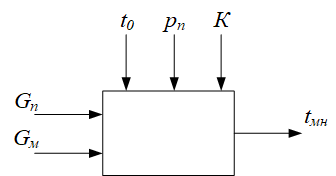
\includegraphics{images/chapter_2/Pasterizer_heat_section.png}
    \caption{Структурная схема секции нагрева ПОУ как объекта автоматизации}
    \label{fig:Pasterizer_heat_section}
\end{figure}

Основными причинами, вызывающими колебания температуры $t_\text{мн}$ нагревания молока являются непостоянство расхода $G_\text{м}$ продукта, непостоянство температуры $t_0$ исходного молока, изменение расхода $G_\text{п}$ пара, обусловленное колебания его давления $p_\text{п}$, изменение коэффициента теплопередачи $K$ вследствие отложения белка молока на теплопередающих поверхностях \cite{Вайнберг1978}.

Для стабилизации температуры $t_\text{мн}$ нагревания молока в качестве управляющего воздействия в основном применяют расход пара $G_\text{п}$. Его регулируют посредством управляемого клапана (\textbf{VC1} на рис. \ref{fig:Pasterizer_heat_section}).

Статические и динамические характеристики большинства ПОУ в настоящее время экспериментально и аналитически выявлены. Для нагревательной части по каналу $G_\text{п} \rightarrow t_\text{мн}$, т. е. зависимость $t_\text{мн}=F(G_\text{п})$ определяется из уравнения теплового баланса секции пастеризации и систем обогрева горячей воды. Если пренебречь потерями тепла в окружающую среду, то уравнение теплового баланса в установившемся режиме имеет вид:

\begin{equation}
    G_\text{м} c_\text{м}(1 - \varepsilon)(t_\text{мн} - t_0) = G_\text{п}(i - c_\text{к} t_\text{к}),
\end{equation}

где $c_\text{к}$ – температура конденсата \SI{}{\celsius}; $c_\text{м}$, $c_\text{к}$ – теплоемкость соответственно молока и конденсата, Дж/(кг·\SI{}{\celsius}); $\varepsilon$ – коэффициент регенерации тепла установки; $i$ – энтальпия пара, Дж/кг. После преобразования данного уравнения получаем статическую характеристику нагревательной части установки:

\begin{equation}
    t_\text{мн} = t_0 + \frac{i - c_\text{к} t_\text{к}}{G_\text{м} c_\text{м}(1 - \varepsilon)} G_\text{п}.
\end{equation}

Результаты экспериментальных и теоретических исследований показали, что динамическая характеристика нагревательной части установки по каналу «расход пара – температура нагрева молока» может быть выражена передаточной функцией:

\begin{equation}\label{steam_temp_relation}
    W(p) = \frac{K_\text{п} e^{-p \tau_\text{з}}} {Tp + 1},
\end{equation}

где $K_\text{п}$ – коэффициент передачи объекта, \SI{}{\celsius}/(кг/с),

\begin{equation}
    K_\text{п} = \frac{i - c_\text{к} t_\text{к}}{G_\text{м} c_\text{м}(1 - \varepsilon)},
\end{equation}

где $T$ – постоянная времени объекта, с; $\tau_\text{з}$ – время запаздывания, с; $p$ – комплексная переменная (оператор Лапласа).

Таким образом, передаточная функция нагревательной части установки характеризуется последовательно соединенными апериодическим звеном первого порядка и звеном транспортного запаздывания. В таблице \ref{table:pasterizer_params} приведены средние значения параметров некоторых ПОУ.

\begin{table} [H]
    \small
    \caption{Параметры ПОУ}\label{table:pasterizer_params}
    \centering
    \begin{tabular}{ | c | c | c | c | }
        \hline
        \textbf{Установка} & $K_\text{п}$, \SI{}{\celsius}/(кг/с) & $T$, c & $\tau_\text{з}$, c \\
        \hline
        ОПУ-5М             & 2300                                 & 369    & 12                 \\
        \hline
        ОПУ-10             & 1150                                 & 190    & 7                  \\
        \hline
        ОПУ-25             & 525                                  & 450    & 4                  \\
        \hline
    \end{tabular}
\end{table}

При накоплении белковых веществ на теплопередающих поверхностях значения $T$ в среднем возрастают на 50 - 60\%.

\subsection{Компьютерное моделирование процесса пастеризации}

Для компьютерного моделирования получим дискретную модель процесса пастеризации на основе формулы (\ref{steam_temp_relation}).

Рассмотрим процесс без участия звена запаздывания $e^{-p \tau_\text{з}}$, положим $k = K_\text{п}$. Выберем достаточно малый шаг времени $h$ и будем вычислять значения сигналов на выходе в дискретные равноотстоящие моменты времени $t = hl$ $(l = 0, 1, 2, \ldots)$. Выходную величину определим по рекуррентным формулам квадратичной интерполяции на основе значений сигнала, полученных в предыдущие моменты времени. Дифференциальное уравнение процесса в интервале $(l - 1)h < t \le hl$ имеет вид:

\begin{equation}
    Tdy(\tau)/d\tau + y(\tau) = kx(\tau),
\end{equation}

где $\tau = t - (l - 1)h$.

При $\tau = 0$ значения $x[(l - 1)h] = x_{l - 1}, y[(l - 1)h] = y_{l - 1}$.

Переходя к изображениям по Лапласу и решая уравнение относительно $Y(p)$, получим:

\begin{equation}
    Y(p) = \frac{1}{1 + pT}y_{l - 1}+\frac{k}{1 + pT}[X(p) - x_{l - 1}].
\end{equation}

При использовании квадратичной интерполяции сигнал $x(t)$ в интервале $[(l - 1)h, lh]$ определяется значениями $x$ для трех моментов времени $x_l = x(lh), x_{l - 1} = x[(l - 1)h)]$ и $x_{l - 2} = x[(l - 2)h)]$, т.е.:

\begin{equation}
    x(t) = x_{l - 1} + \frac{x_l - x_{l - 2}}{2h} + \frac{x_l - 2x_{l - 1}+ x_{l - 2}}{h^2},
\end{equation}

или в изображениях:

\begin{equation}
    x(p) = \frac{x_{l - 1}}{p} + \frac{x_l - x_{l - 2}}{2h}\cdot\frac{1}{p^2} + \frac{x_l - 2x_{l - 1} + x_{l - 2}}{h^2}\cdot\frac{1}{p^3}.
\end{equation}

Выполняя подстановку и обратное преобразование Лапласа, при $\tau = h$, т.е. в конце интервала $(t = lh)$, имеем:

\begin{equation}
    y_l = \gamma y_{l - 1} + Ax_l + Bx_{l - 1} + Cx_{l - 2},
\end{equation}

где:

\begin{equation}
    \begin{rcases}
        \gamma = e^{-h/T};\\
        A = \frac{k}{2h^2}[(1 - \gamma)(2T^2 - Th) + 2h^2 - 2Th];\\
        B = -\frac{k}{h^2}[(1 - \gamma)(2T^2 - h^2) + h^2 - 2Th];\\
        C = \frac{k}{2h^2}[(1 - \gamma)(2T^2 + Th) - 2Th].
    \end{rcases}
\end{equation}

С учетом запаздывания $\tau_\text{з}$ получим \cite{Нетушил1978}:

\begin{equation}
    y_l = \gamma y_{l - 1} + Ax_{l - \tau_\text{з}} + Bx_{l - \tau_\text{з} - 1} + Cx_{l - \tau_\text{з} - 2}.
\end{equation}.

\subsection{Разработанный нейро-ПИД регулятор ПОУ}

Общая структура самонастраивающегося нейро-ПИД регулятора показана на рисунке \ref{fig:neuro_PID_controller}, где выходы нейронной сети – пропорциональный ($K$) коэффициент, интегральная ($T_I$) и дифференциальная ($T_D$) составляющие.

\begin{figure}[H]
    \centering
    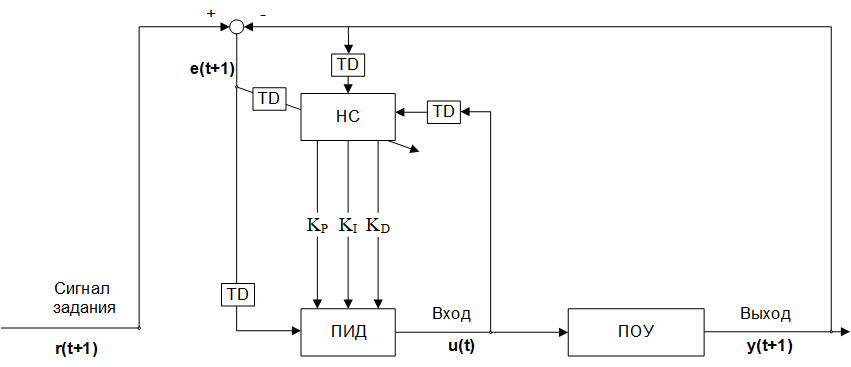
\includegraphics[width=\textwidth]{images/chapter_2/Разработанный нейро-контроллер.png}
    \caption{Разработанный нейро-ПИД-регулятор, TD означает оператор задержки}
    \label{fig:neuro_PID_controller}
\end{figure}

В качестве настройщика ПИД использовался многослойный персептрон (MLP) со следующей структурой: 20 входных, 10 скрытых и 3 выходных нейронных элемента; функция активации скрытого и выходного слоев – сигмоидная (рис. \ref{fig:PID_neuro_tuner}).

\begin{figure}[H]
    \centering
    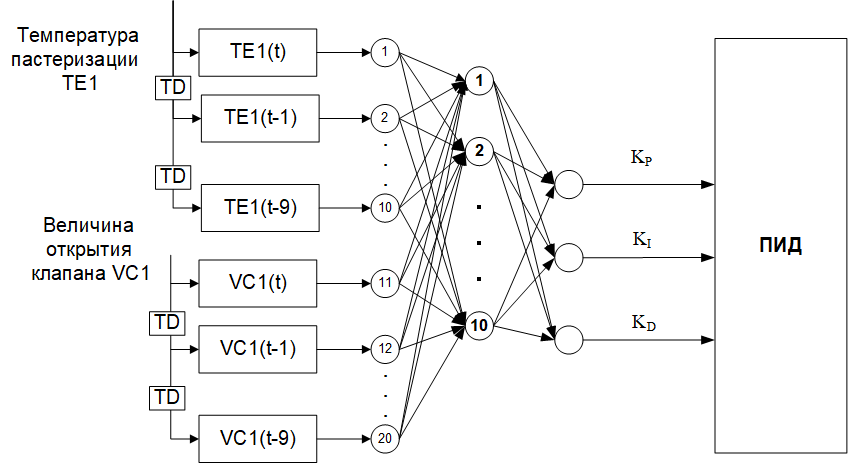
\includegraphics[width=\textwidth]{images/chapter_2/Нейро-настройщик ПИД.png}
    \caption{Нейро-настройщик ПИД}
    \label{fig:PID_neuro_tuner}
\end{figure}

\subsection{Алгоритм функционирования нейро-ПИД регулятора}

ПИД-регулятор в дискретном времени можно описать выражением \ref{PID_algorithm}, где $P$, $T_I$ и $T_D$ – пропорциональный коэффициент, интегральная и дифференциальная составляющие соответственно, $u_n$ определяет вход объекта управления в момент времени $t = n T_0$ и $e_n$ – ошибка между желаемым значением выхода $r_n$ и реальным, то есть $e_n = r_n - y_n$. $T_0$ определяет единичный интервал времени.

Для использования алгоритма обратного распространения ошибки мы должны выбрать функцию $E$, значение которой должно быть минимизировано. В качестве такой функции будет выступать ошибка управления $e_n$ в момент времени $t = n T_0$ - получаем $E_n = \frac{1}{2}e_n^2$.
Для накопления ошибок сохраняем полученные ранее данные – $E_{n-p},...E_{n-2},E_{n-1},E_n$, где $p$ определяет количество сохраненных ранее образов, используемых для обучения сети.

